\chapter{Gaussian Mixture Models}
\label{cap:gmm}

In this chapter, we will review fundamental concepts of Gaussian Mixture Models (GMMs) and introduce some notations that will be used throughout this dissertation (Sections \ref{sec:gmm:fundamentals} and \ref{sec:gmm:models}). We will then discuss the literature on the number of modes (local maxima) in GMMs (Section \ref{sec:gmm:nmodes}) and, finally, approaches to find such modes (Section \ref{sec:gmm:fmodes}).

We assume some basic knowledge of probabily theory; gentle introductions are found in the works of \citet{Jaynes2003} and \citet{Kadane2011}.

\section{Gaussian distribution}
\label{sec:gmm:fundamentals}

We will use uppercase letters to denote random variables (RVs) and lowercase letters to denote assignments of RVs.

\begin{definition}[Univariate Gaussian]
  An RV $X$ has a \textbf{univariate Gaussian distribution} with mean $\mu$ and variance $\sigma^2$, denoted $X \sim \mathcal{N}\left(\mu, \sigma^2\right)$, if it has the probability density function

  \begin{equation}
    p(x) = \frac{1}{\sqrt{2\pi} \sigma} e^{-\frac{(x - \mu)^2}{2\sigma^2}} \, .
  \end{equation}
\end{definition}

\noindent We will use $p( \cdot )$ to denote probability density functions (PDFs). Figure \ref{fig:gaussian}(a) shows the PDFs of three univariate Gaussian distributions.

\begin{figure}
  \begin{minipage}{0.5\textwidth}
    \centering
    \scalebox{0.8}{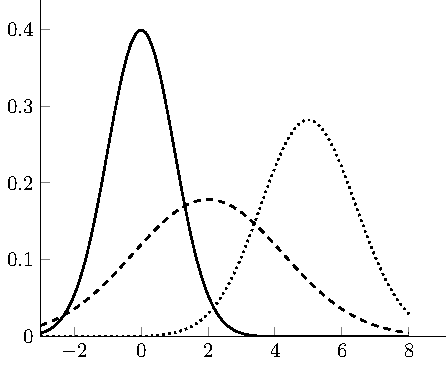
\includegraphics{figures/gaussian-a.pdf}}

    (a)
  \end{minipage}\begin{minipage}{0.5\textwidth}
    \centering
    \scalebox{0.8}{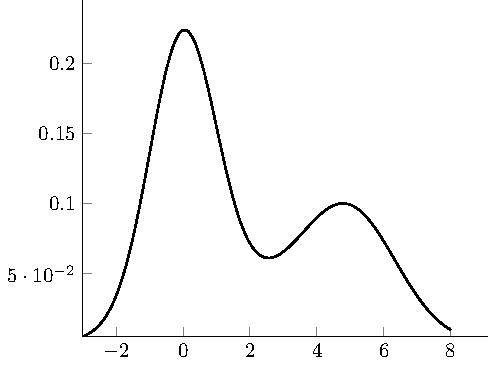
\includegraphics{figures/gaussian-b.pdf}}

    (b)
  \end{minipage}

  \caption[Plot of Gaussian distributions and GMM]{
    \textbf{(a)} Plot of the PDFs of three Gaussian distributions: $\mathcal{N}(0, 1)$ (solid line), $\mathcal{N}(2, 5)$ (dashed line) and $\mathcal{N}(5, 2)$ (dotted line).
    \textbf{(b)} Plot of the PDF of a univariate Gaussian mixture model, $X \sim 0.5 \mathcal{N}(0, 1) + 0.2 \mathcal{N}(2, 5) + 0.3 \mathcal{N}(5, 2)$.
  }
  \label{fig:gaussian}
\end{figure}

Gaussian distributions are extended to the multivariate case:

\begin{definition}[Multivariate Gaussian]
  A random vector $\mathbf{X} = (X_1, \cdots, X_n)$ is said to have a \textbf{multivariate Gaussian distribution} with mean $\boldsymbol{\mu}$ (a $n$-dimensional vector) and covariance matrix $\boldsymbol{\Sigma}$ (to not be confused with summation sign), $\mathbf{X} \sim \mathcal{N}\left(\boldsymbol{\mu}, \boldsymbol{\Sigma}\right)$, if:

  \begin{equation}
    p(\mathbf{x}) = 2\pi^{-\frac{n}{2}} \textrm{det}\left(\boldsymbol{\Sigma}\right)^{\frac{1}{2}} e^{-\frac{1}{2}\left(\mathbf{x}-\boldsymbol{\mu}\right)^T\boldsymbol{\Sigma}^{-1}\left(\mathbf{x}-\boldsymbol{\mu}\right)} \, .
  \end{equation}
\end{definition}

\noindent We will denote random vectors using bold uppercase letters and assignments of random vectors using bold lowercase letters. Random vectors and sets of random variables will be used interchangeably for the sake of simplicity in notation.

$\boldsymbol{\Sigma}$ is a symmetric $n \times n$ matrix and the value $\Sigma_{i,j}$ is, by definition, the covariance between variables $X_i$ and $X_j$, $\operatorname{Cov}[X_i, X_j]$:

\begin{equation}
  \Sigma_{i,j} := \operatorname{Cov}[X_i, X_j] = \operatorname{E}\left[(X_i - \mu_i)( X_j - \mu_j)\right] \, .
\end{equation}

In general, RVs may be uncorrelated but statistically dependent. In the case of multivariate Gaussian distributions, two or more variables are uncorrelated if and only if they are independent. The product of PDFs of independent Gaussian RVs is a multivariate Gaussian distribution with a diagonal covariance matrix.

A Gaussian distribution is said to be \textbf{isotropic} (or \emph{spherical}) if its covariance matrix is diagonal and all variables have the same variance. Formally, a distribution in $\mathbb{R}^d$ is isotropic if $\mathbf{\Sigma} = \sigma^2\mathbf{I}_d$ for some $\sigma \in \mathbb{R}$, where $\mathbf{I}_d$ is the identity matrix of size $d$.

\section{Mixture models}
\label{sec:gmm:models}

A finite \textbf{mixture model} is a distribution formed by a convex combination of distributions. Formally, if $p_1(\mathbf{X}), \cdots, p_n(\mathbf{X})$ are densities over a random vector $\mathbf{X}$, we can define a finite mixture model $p(\mathbf{X})$ of components $p_1, \cdots, p_n$ by choosing weights $w_1, \cdots, w_n \geq 0$ such that $\sum_{z=1}^n w_z = 1$ and making:

\begin{equation}
  p(\mathbf{x}) = \sum_{z=1}^n w_z p_z(\mathbf{x}) \, .
\end{equation}

We can interpret the mixture coefficients $w_z$ as a categorical \textbf{latent variable} (usually denoted $Z$) such that $p(z) = w_z$, $p(\mathbf{x} \mid z) = p_z(\mathbf{x})$, and

\begin{equation}
  p(z, \mathbf{x}) = p(z) p(\mathbf{x} \mid z) \, .
\end{equation}

\noindent Variables in $\mathbf{X}$ are called \textbf{observable variables} in contrast to latent variables. Then, computing $p(\mathbf{x})$ consists in marginalizing the variable $z$:

\begin{eqnarray}
  p(\mathbf{x}) & = & \sum_{z=1}^n p(z) p(\mathbf{x}, z) \\
  & = & \sum_{z=1}^n w_z p_z(\mathbf{x}) \, .
\end{eqnarray}

\begin{definition}[Gaussian Mixture]
  A \textbf{Gaussian Mixture Model} (GMM) is a mixture model of Gaussian distributions.
\end{definition}

\noindent Figure \ref{fig:gaussian}(b) depicts a univariate GMM, but in this work, we will mainly deal with multivariate GMMs.

A GMM is said to be \textbf{homoscedastic} if it has equal covariance matrices for all its components, and is said to be \textbf{isotropic} if its components are isotropic.

\section{Number of modes}
\label{sec:gmm:nmodes}

The \textbf{modes}, or local maxima, of a density in $d$ dimensions are the points of the PDF at which it achieves a local maximum value.

\begin{definition}[Mode]
  A point $\mathbf{x}^\star \in \mathbb{R}^d$ is a mode of $f(\mathbf{x})$ if there exists a neighborhood\footnote{Given a $\delta > 0$, a \emph{neighborhood} of $\mathbf{x}^\star$ is the set of points $\mathbf{x} \in \mathbb{R}^d$ which satisfy $||\mathbf{x}^\star - \mathbf{x}||_2 < \delta$.} of $\mathbf{x}^\star$ such that $f(\mathbf{x}^\star) \geq f(\mathbf{x})$ for all $\mathbf{x}$ within that neighborhood.
\end{definition}

While a probability distribution can have multiple modes (for example, uniform distributions have infinitely many modes), a Gaussian distribution has only one mode, namely, its mean. At first glance, one might assume that the number of modes of a GMM would be small and easy to determine, since it is a combination of a finite number of Gaussian components. However, the number of modes that a mixture of $k$ Gaussians in $\mathbb{R}^d$ can possess is surprisingly unknown, not proven to be finite, and identifying such modes remains a challenging problem.

Let $m(d, k)$ denote the maximal number of modes for $d$-dimensional Gaussian mixtures with $k$ components. As previously stated, $m(d, 1) = 1$, because a GMM with one component is simply a Gaussian distribution. Numerous studies have examined the lower and upper bounds of $m(d, k)$ for greater values of $d$ and $k$, and we will briefly review some of the most recent ones, such as the ones by \citet{Carreira-Perpinan2003a}, \citet{Ray2012}, and \citet{Amendola2019}.

While \citet{Carreira-Perpinan2003} proved that the number of modes of univariate GMMs is limited by its number of components ($m(1, k) = k$), the result does not hold in higher dimensions. Figure \ref{fig:amendola}(a) presents a counterexample that shows the mixture of two Gaussians in two dimensions, $\mathbf{X}_1 \sim \mathcal{N}\left(\boldsymbol{\mu}_1, \boldsymbol{\Sigma}_1\right)$ and $\mathbf{X}_2 \sim \mathcal{N}\left(\boldsymbol{\mu}_2, \boldsymbol{\Sigma}_2\right)$, where $\boldsymbol{\mu}_1 = (1, 0)$, $\boldsymbol{\Sigma}_1 = [(1, 0), (0, 0.1)]$, $\boldsymbol{\mu}_2 = (0, 1)$, and $\boldsymbol{\Sigma}_2 = [(0.1, 0), (0, 1)]$, with coefficients $w_1 = w_2 = \frac{1}{2}$. The mixture has two modes near the original means at $(1, 0)$ and $(0, 1)$, and a third mode near the origin.

\begin{figure}
  \begin{minipage}{0.3333\textwidth}
    \centering
    \scalebox{0.085}{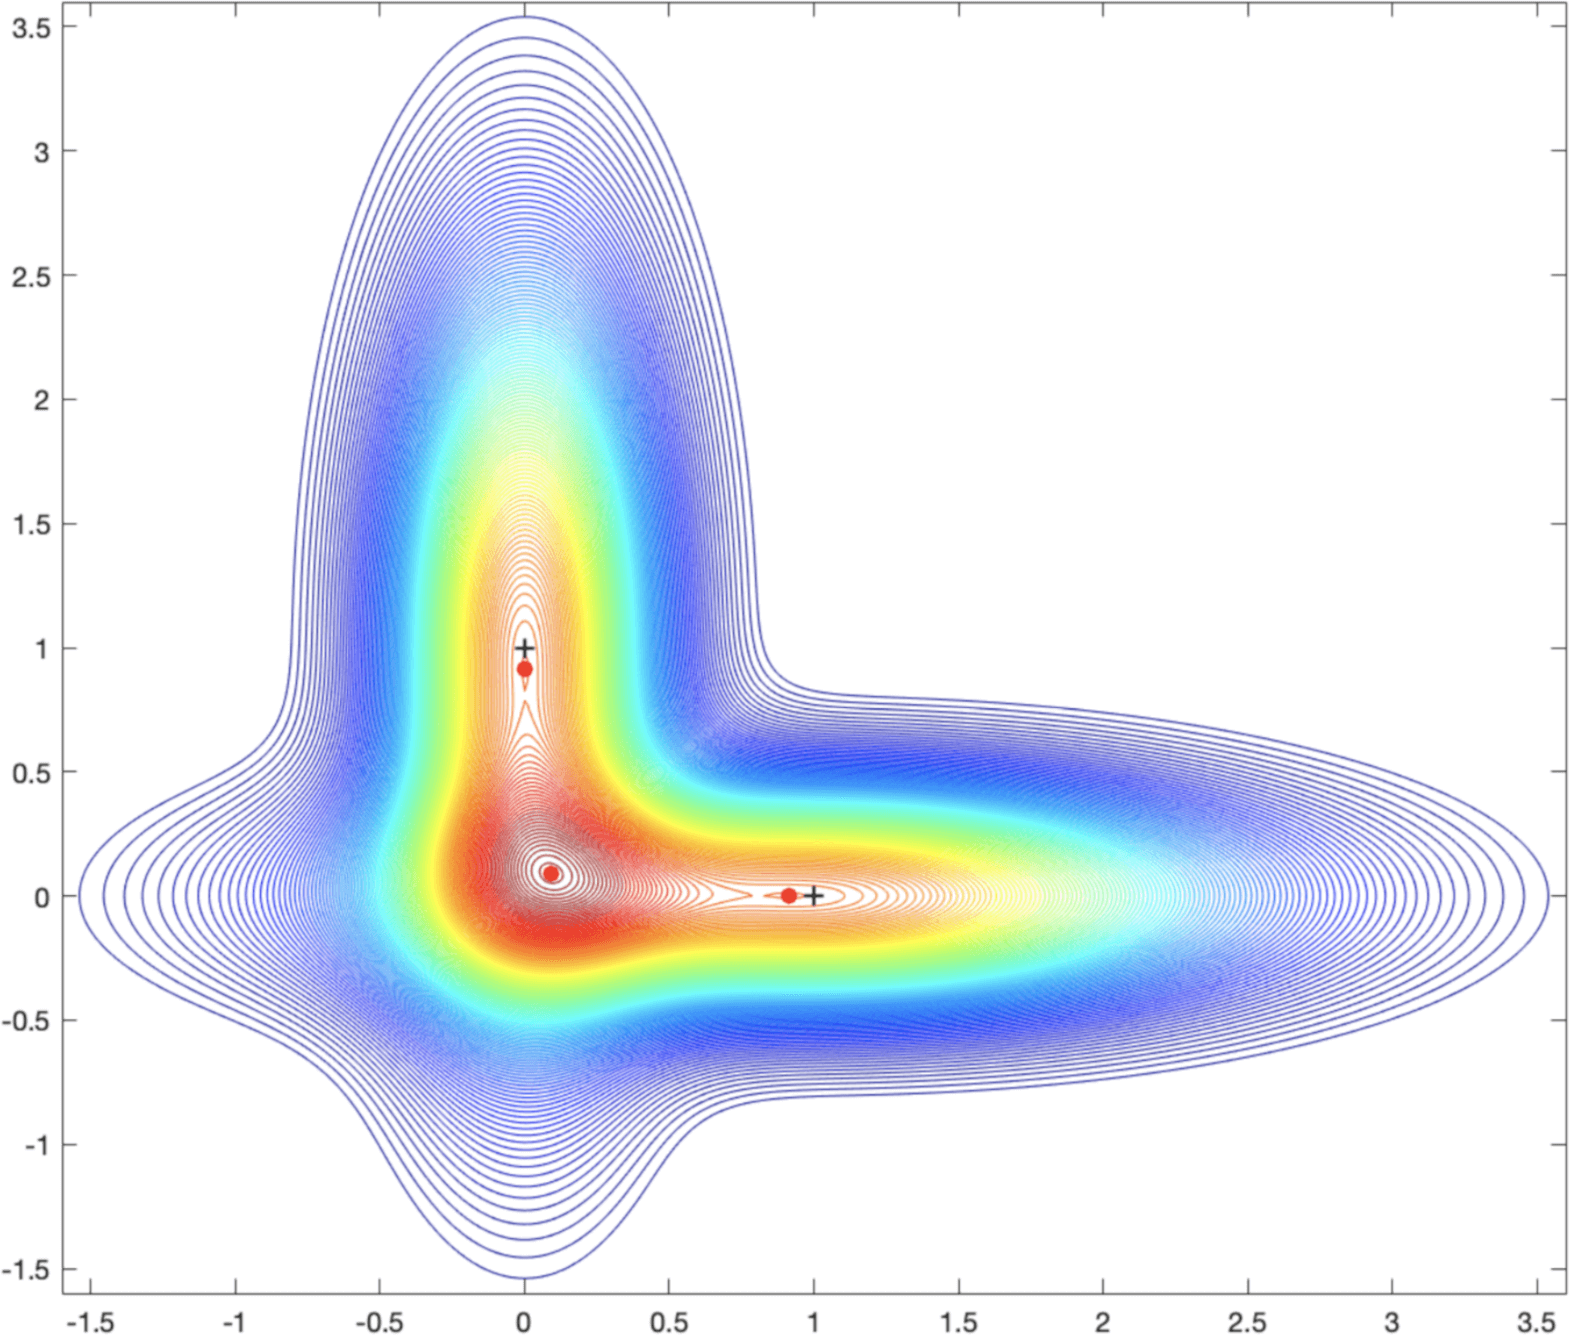
\includegraphics{figures/amendola1.png}}

    (a)
  \end{minipage}\begin{minipage}{0.3333\textwidth}
    \centering
    \scalebox{0.085}{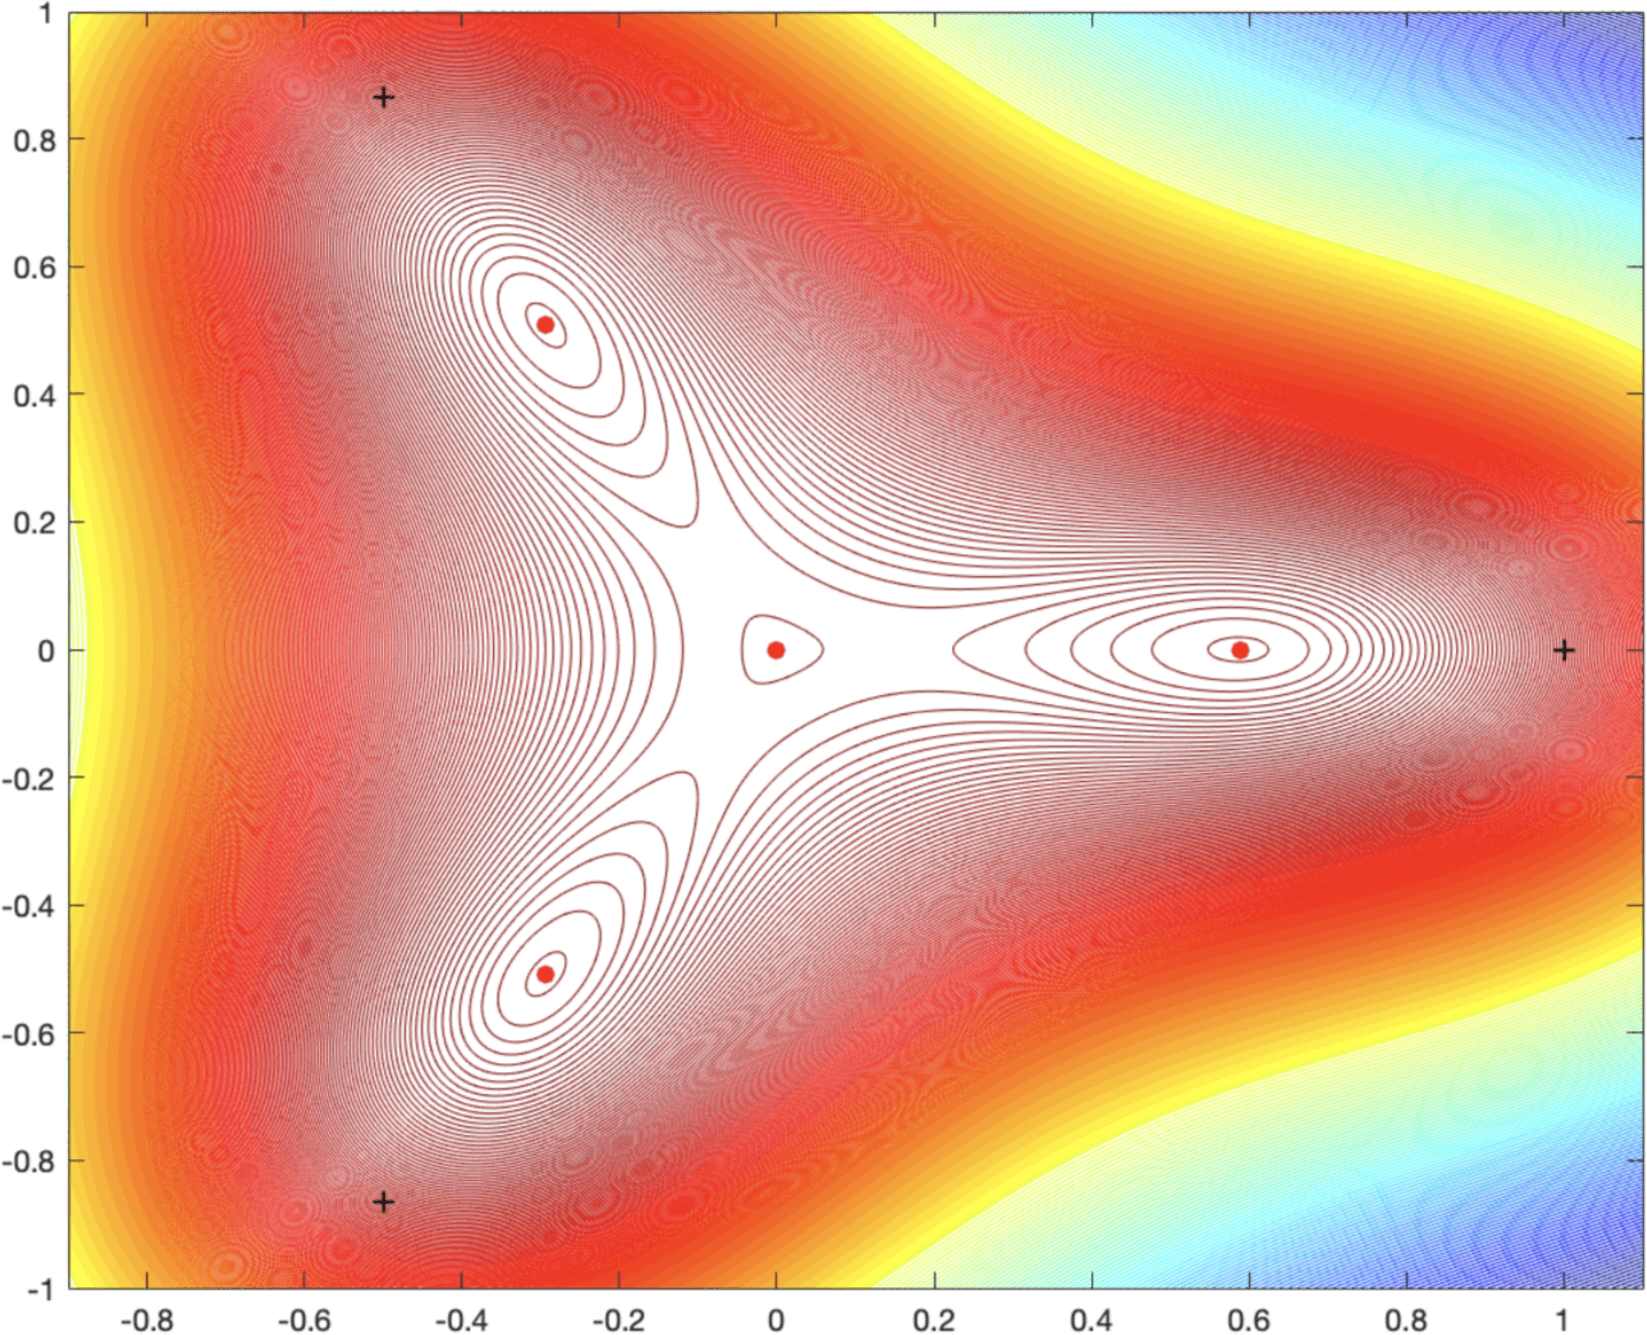
\includegraphics{figures/amendola2.png}}

    (b)
  \end{minipage}\begin{minipage}{0.3333\textwidth}
    \centering
    \scalebox{0.085}{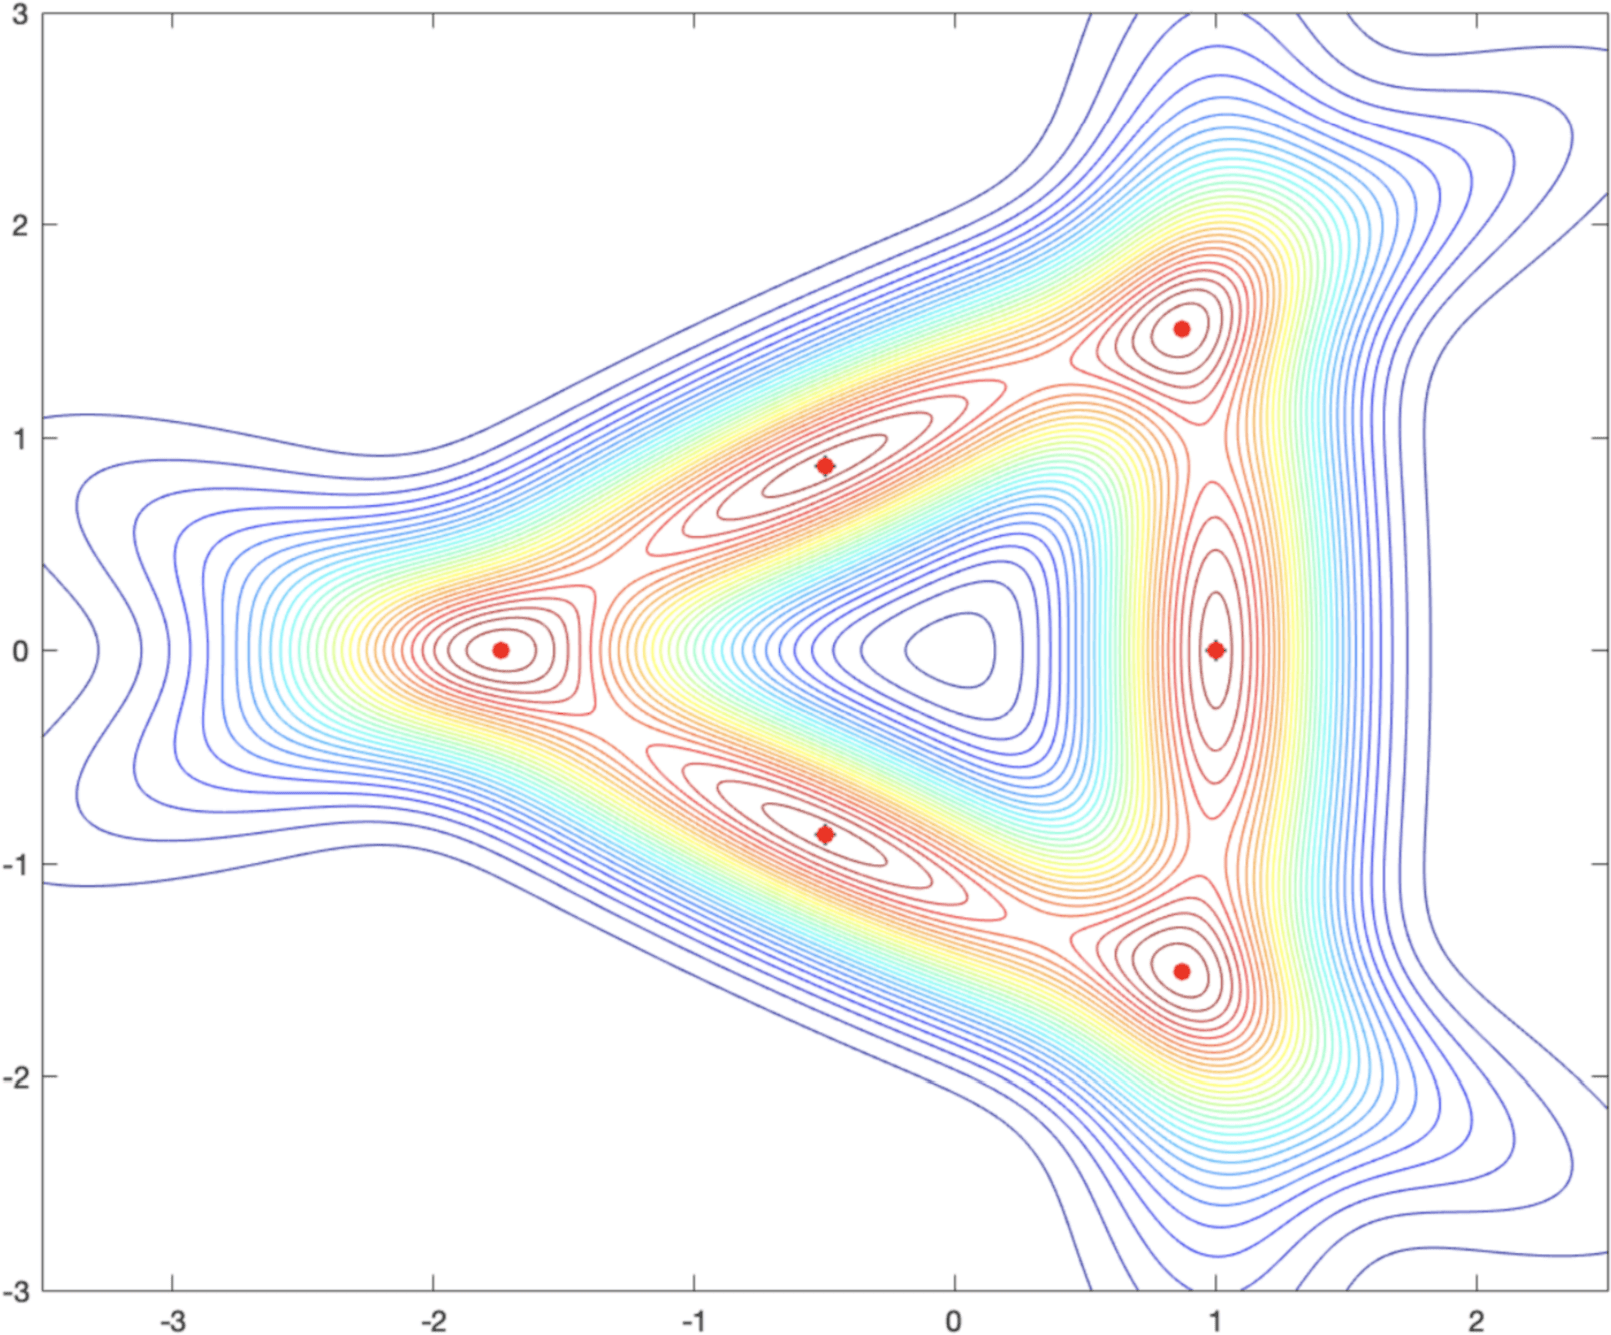
\includegraphics{figures/amendola3.png}}

    (c)
  \end{minipage}

  \caption[Bivariate GMMs with more modes than components]{
    Bivariate GMMs with more modes than components. Component means are represented by $+$ (black crosses) and GMM modes are represented by {\color{red} $\bullet$} (red bullets).
    \textbf{(a)} 2 components and 3 modes.
    \textbf{(b)} 3 isotropic components and 4 modes.
    \textbf{(c)} 3 components and 6 modes.
    Source: \citet{Amendola2019}.
  }
  \label{fig:amendola}
\end{figure}

In a conjecture, the same article suggested that the number of modes of an isotropic GMM could not exceed its number of components. However, a counterexample presented by J. J. Duistermaat \citep{Carreira-Perpinan2003a} proved that conjecture to be false. The counterexample, shown in Figure \ref{fig:amendola}(b), consists of an homoscedastic isotropic GMM with three components positioned at the vertices of an equilateral triangle and four modes. The mixture is formed by $\mathbf{X}_1 \sim \mathcal{N}\left((1, 0), \sigma^2I_2\right)$, $\mathbf{X}_2 \sim \mathcal{N}\left(\left(-\frac{1}{2}, \frac{\sqrt{3}}{2}\right), \sigma^2I_2\right)$, and $\mathbf{X}_3 \sim \mathcal{N}\left(\left(-\frac{1}{2}, -\frac{\sqrt{3}}{2}\right), \sigma^2\mathbf{I}_2\right)$, where $\sigma^2 = 0.53$, $\mathbf{I}_2$ is the identity matrix of size $2 \times 2$, and $w_1 = w_2 = w_3 = \frac{1}{3}$.

\citet{Ray2012} proved that one can get as many as $d+1$ modes from a Gaussian mixture of two components in $\mathbb{R}^d$ and that is always possible to find a GMM of only two components with $d+1$ modes in $d$ dimensions, therefore $m(d, 2) = d+1$. GMMs with more components can get much more complex. To give an example, Figure \ref{fig:amendola}(c) shows a GMM in $\mathbb{R}^2$ with 3 components and 6 modes, demonstrating that $m(2, 3) \geq 6$.

To date, the most stringent lower and upper bounds for $m(d, k)$ were established by \citet{Amendola2019}. They demonstrate that, given integers $k, d \geq 2$, there exists a mixture of $k$ Gaussians in $d$ dimensions with at least ${k \choose d} + k$ modes, i.e., $m(d, k) \geq {k \choose d} + k$. Additionally, they prove that the number of non-degenerate stationary points for a GMM with $k$ components in $d$ dimensions is bounded by $2^{d+{k \choose 2}}(5+3d)^k$. That means that, assuming that every mixture of $k$ Gaussians in $\mathbb{R}^d$ has finitely many modes, then

\begin{equation}
  {k \choose d} + k \, \leq \, m(d, k) \, \leq \, 2^{d+{k \choose 2}}\left(5+3d\right)^k.
\end{equation}

That result shows that the lower bound for the number of modes in a GMM is unexpectedly large, especially for mixtures with many components. For instance, this bound implies that there exists a GMM with 100 components in $\mathbb{R}^{50}$ with more than $10^{29}$ modes, a fact that seems counterintuitive.

It is also surprising that there is still no conclusive evidence as to whether the number of modes of a GMM is always finite. Although it may seem intuitive that a finite mixture of Gaussians would not contain non-degenerate critical points, the lack of proof leaves the possibility that there may not exist a finite upper bound for $m(k, d)$.

Nevertheless, it is important to note that in real-life scenarios, the number of modes of GMMs does not seem to explode, at least when the components are isotropic. According to \citet{Carreira-Perpinan2003a}, it is very rare to find GMMs with more modes than components in such cases.

\section{Finding modes of GMMs}
\label{sec:gmm:fmodes}

The results regarding the number of modes of GMMs provide insight into the intricate nature of the modes landscape. In this study, we investigate how to find modes of GMMs, and two fundamental initial questions are: (1) where are the modes located, and (2) which specific modes we aim to find.

On the question of \emph{where are the modes located}, for isotropic GMMs it is proven that the modes lie inside the convex hull of the component centroids \citep{Amendola2019}. However, this property does not hold for non-isotropic GMMs, as illustrated by a counter-example in $\mathbb{R}^2$ shown in \ref{fig:amendola}(a).

As an exercise of imagination, we propose the conjecture that, in general, the modes of a GMM reside within the hyperrectangle formed by the minimum and maximum values of each coordinate in the component centroids. Even if that is not always true, we can argue that such modes have greater practical relevance: the primary applications of finding modes of GMMs are either finding probable values of a model or, notably, clustering in domains such as data analysis, pattern recognition and image processing. In this context, a mode is considered a representative of a cluster, and a mode located outside the space between the centroids may not be a suitable representative for a cluster.

As for \emph{which specific modes we aim to find}, it is usually not crucial to identify all the modes of a model, but rather the most probable one or modes to which data points converge. That led us to investigate two problems: finding global maxima and finding modes starting from points.

\vspace{1em}

Starting with global maxima, seeking such mode has applications such as real-time object tracking in computer vision \citep{Shen2005} and has been investigated by \citet{Pulkkinen2014} in his PhD thesis.

\citet{Pulkkinen2013} introduced a method for smoothing a given GMM using Gaussian convolution. This technique effectively eliminates undesired local maxima while preserving the fundamental structure of the GMM. The convolved Gaussian mixture has been shown to be strictly concave under mild assumptions, and therefore has a unique maximum. Notably, their proposed method operates globally, meaning it is not dependent on the starting point, and has the ability to identify a significant mode, although not necessarily the maximum one. In the same paper, the authors argued that finding the global mode of a Gaussian kernel density estimate, which is a special case of a Gaussian mixture, is a difficult global optimization problem.

\vspace{1em}

Finding multiple modes starting from points is usually done using hill-climbing methods, which are designed to iteratively ascend from any initial point. We will briefly review Gradient Ascent, Mean-Shift and Modal EM.

\subsubsection{Gradient ascent}

For differentiable functions, \textbf{Gradient Ascent} \citep{Murphy2012} is a popular iterative optimization algorithm to find a mode. At each step, the algorithm computes the gradient of the function at the current point ($\mathbf{x}^{(r)}$) and updates the point in the direction of the gradient: $\mathbf{x}^{(r+1)} \gets \mathbf{x}^{(r)} + \gamma \nabla f\left(\mathbf{x}^{(r)}\right)$. However, a major issue with this method is that it heavily relies on the choice of a step size parameter, $\gamma \in \mathbb{R}+$, which must be carefully selected to ensure that $f\left(\mathbf{x}^{(r+1)}\right) \geq f\left(\mathbf{x}^{(r)}\right)$ for all $r$. Finding an appropriate step size can be a difficult and costly process, as it often requires multiple iterations of its own. This can make Gradient Ascent slow to converge.

\subsubsection{Mean-Shift}

In the field of cluster analysis, a common technique to locate the modes of a density is \textbf{Mean-Shift} and its variants \citep{Fukunaga1975, Carreira-Perpinan2015}. Traditionally, the Mean-Shift algorithm does not take a model (density function) as input. Instead, it works directly with data points by defining a kernel density estimate, making it suitable for clustering since the input is similar to that of other clustering algorithms such as $k$-means (except for not requiring a $k$ parameter). The algorithm iteratively shifts a point to the average of data points in its neighborhood until the point does not change.

Formally, let data be a finite set $\mathbf{S} = \left\{\mathbf{s}_n\right\}_{n=1}^N \subset \mathbb{R}^d$, so that a $\mathbf{s} \in \mathbf{S}$ corresponds to a single data point in $\mathbb{R}^d$. Let $\mathbf{x}^{(0)}$ be a point in $\mathbb{R}^d$. The \textbf{sample mean} at $\mathbf{x}$ is defined as:

\begin{equation}
  m\left(\mathbf{x}\right) := \frac{
    \sum_{\mathbf{s} \in \mathbf{S}} K\left(\mathbf{s}-\mathbf{x}\right) \mathbf{s}
  }{
    \sum_{\mathbf{s} \in \mathbf{S}} K\left(\mathbf{s}-\mathbf{x}\right)
  } \, ,
\end{equation}

\noindent where $K(\mathbf{x})$ is a \emph{kernel} function that comprises a bandwidth parameter $\lambda$. Commonly, flat kernels and Gaussian kernels have been used. A \textbf{flat kernel} is the characteristic function $F$ of the $\lambda$-ball in $\mathbb{R}^d$:

\begin{equation}
  F(\mathbf{x}) := \begin{cases}
    1 & \text{ if } ||\mathbf{x}|| \leq \lambda \, , \\
    0 & \text{ if } ||\mathbf{x}|| > \lambda \, ,
  \end{cases}
\end{equation}

\noindent and a \textbf{Gaussian kernel} is defined as:

\begin{equation}
  G(\mathbf{x}) := e^{-\frac{||\mathbf{x}||^2}{2\lambda^2}} \, .
\end{equation}

\noindent (In this case the parameter $\lambda$ is the standard deviation of the Gaussian function, normally denoted as $\sigma$).

The difference $m(\mathbf{x}) - \mathbf{x}$ is called \textbf{mean shift vector} and, at each step, the Mean-Shift algorithm updates the point in its direction, making $\mathbf{x}^{(r+1)} \leftarrow m\left(\mathbf{x}^{(r)}\right)$.

Mean-Shift has been re-discovered, adapted and modified for various density functions in several studies \citep{Cheng1995, Carreira-Perpinan2000, Comaniciu2002}. The algorithm was extended to use mixture components instead of kernel density estimation from data points. In the case of Gaussian Mixture Models, it has been demonstrated that the Mean-Shift algorithm is equivalent to a Expectation-Maximization method named Modal EM \citep{Carreira-Perpinan2007, Chacon2019}, which we will describe next.

\subsubsection{Modal EM}

\citet{Carreira-Perpinan2000} proposed another fixed-point iterative schema as follows. Given a GMM $p(\mathbf{x}) = \sum_{z=1}^n w_z p_z(\mathbf{x})$ and a point $\mathbf{x}^{(r)}$,

\begin{equation}
  \label{eq:mem:gmm}
  \mathbf{x}^{(r+1)} \gets \frac{
  \sum_{z=1}^n w_z p_z\left(\mathbf{x}^{(r)}\right) \boldsymbol{\Sigma}_z^{-1} \boldsymbol{\mu}_z
  }{
  \sum_{z=1}^n w_z p_z\left(\mathbf{x}^{(r)}\right) \boldsymbol{\Sigma}_z^{-1}
  } \, .
\end{equation}

\noindent This algorithm has some advantages over Gradient Ascent, such as not requiring any additional parameters. Additionally, it was shown to be a Expectation-Maximization (EM) method, which facilitates its convergence analysis. As such, it approaches a mode from almost any initial point and monotonically increases the density value or leaves it unchanged: $p(\mathbf{x}^{(r+1)}) \geq p(\mathbf{x}^{(r)})$, and $\mathbf{x}^{(r+1)} \neq \mathbf{x}^{(r)} \Rightarrow p(\mathbf{x}^{(r+1)}) > p(\mathbf{x}^{(r)})$.

Independently, \citet{Li2007} introduced an EM-style method named \textbf{Modal EM} which is equivalent to the schema proposed by \citet{Carreira-Perpinan2000} for GMMs, as we will observe in Chapter \ref{cap:algorithm}. To apply Modal EM, one starts with a mixture density of $\tau$ components, $p(\mathbf{x}) = \sum_k^\tau w_k p^k(\mathbf{x})$, and an initial point $\mathbf{x}^{(0)}$. The method then alternates between the following two steps, starting with $r = 0$:

\begin{equation}
  \label{eq:mem:expectation}
  \text{\textbf{Expectation}: Let }
  q_k = \frac{w_k p^k\left(\mathbf{x}^{(r)}\right)}{p\left(\mathbf{x}^{(r)}\right)},
  \text{ for } k = 1, \cdots, \tau \, .
\end{equation}

\begin{equation}
  \label{eq:mem:maximization}
  \text{\textbf{Maximization}: Compute }
  \mathbf{x}^{(r+1)} = \arg\max_\mathbf{x} \sum_k^\tau q_k \log p^k\left(\mathbf{x}\right) \, .
\end{equation}
